\section{Special-relativistic convergence and optical-depth transition}\label{sec:sr_regimes}

We first verify spatial convergence order, relativistic multi-stream pairing, and asymptotic collisional crossover on flat three-dimensional periodic domains in normal-observer Cartesian coordinates ($\alpha = 1$, $\beta^i = 0$, $\gamma_{ij} = \delta_{ij}$).

Warm sound-like perturbations test continuum spatial convergence cleanly away from shock discontinuities. Initializing a single relativistic top-hat velocity basis with mean boost $\bar{u}_x = 0.3$, uniform density modulation amplitude $0.05$, and isotropic momentum dispersion $\sigma_u = 0.25$ across moving elements $N \in \{8^3, 12^3, 16^3\}$ yields monotonic $L_1$ error reduction against a $24^3$ continuum reference at $t = 0.08$. Figure~\ref{fig:sr_regimes} (left panel) confirms near second-order convergence under spatial refinement while safeguarded analytical Newton face-speed solves match reference Brent iterations down to sub-part-per-thousand tolerance across mild and ultrarelativistic ($\bar{u}_x = 1.5$) waves with machine-precision rest-mass conservation.

Two-stream interpenetration across a vacuum interface tests boosted face-frame basis pairing against naive coordinate-velocity matching. Two cold-core streams cross obliquely at bulk velocities up to $|\bar{\bm{u}}| = 3$ on a periodic cube while the second stream vanishes outside a sharp slab boundary. Under covariant face-frame pairing, empty velocity slots align cleanly across faces and preserve complete stream separation through $t = 0.40$ without artificial momentum-space broadening, whereas unboosted velocity matching pairs populated bases across the vacuum discontinuity with empty slots and triggers spurious dispersion growth.

\begin{figure}[tbp]
\centering
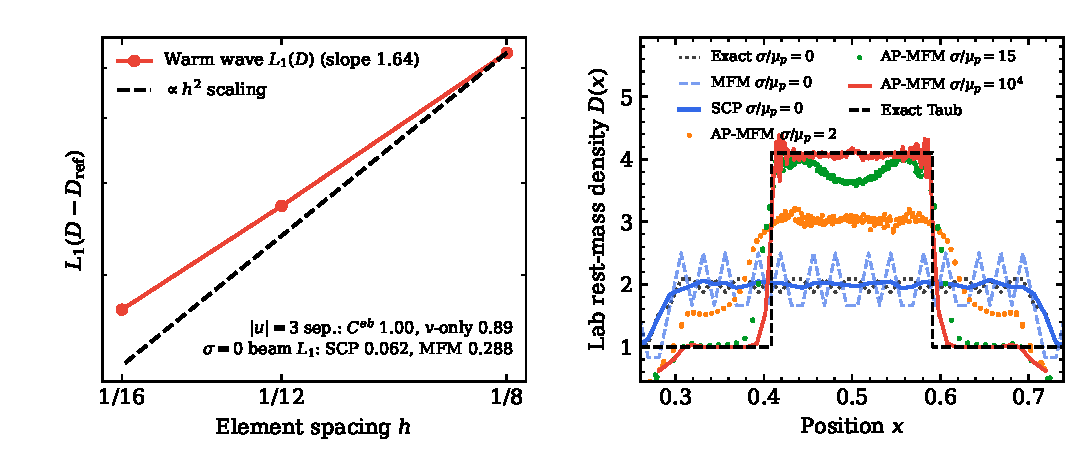
\includegraphics[width=\columnwidth]{figures/fig_sr_regimes.pdf}
\caption{\label{fig:sr_regimes}%
Special-relativistic periodic benchmarks. Left: Warm-wave density error $L_1(D - D_{\rm ref})$ vs spacing $h$, normalized two-stream separation ($|\bar{\bm{u}}|=3$), and collisionless beam $L_1$ error. Right: Colliding-beam density $D(x)$ across $\sigma/\mu_p \in \{0, 2, 15, 10^4\}$ vs exact characteristics and the Taub jump.}
\end{figure}

Three-dimensional colliding beams probe automatic branch switching across four orders of magnitude in dimensionless cross section $\sigma/\mu_p \in \{0, 2, 15, 10^4\}$ for $N = 2400$ two-basis elements at $t = 0.55$. Figure~\ref{fig:sr_regimes} (right panel) compares evolved lab-frame rest-mass density profiles $D(x)$ against a high-resolution $512$-node exact collisionless characteristic solution at $\sigma/\mu_p = 0$ and the analytical relativistic Rankine--Hugoniot Taub jump~\cite{Synge:1957,Mignone:2005ns} at strong coupling. When $\sigma/\mu_p = 0$, the solver dispatches automatically to symplectic cubature packets, expanding populated top-hat bases into $33600$ deterministic characteristics that conserve rest mass and energy to rounding precision and eliminate the counter-streaming oscillations seen in continuum MFM on identical initial elements. At finite collisionality ($\sigma/\mu_p \in \{2, 15, 10^4\}$), continuum MFM coupled with Maxwell--J\"uttner relaxation, asymptotic HLLC Riemann fluxes, and harmonic Noh thermal conduction transitions smoothly toward the analytical Taub compression plateau.

\begin{figure*}[tbp]
\centering
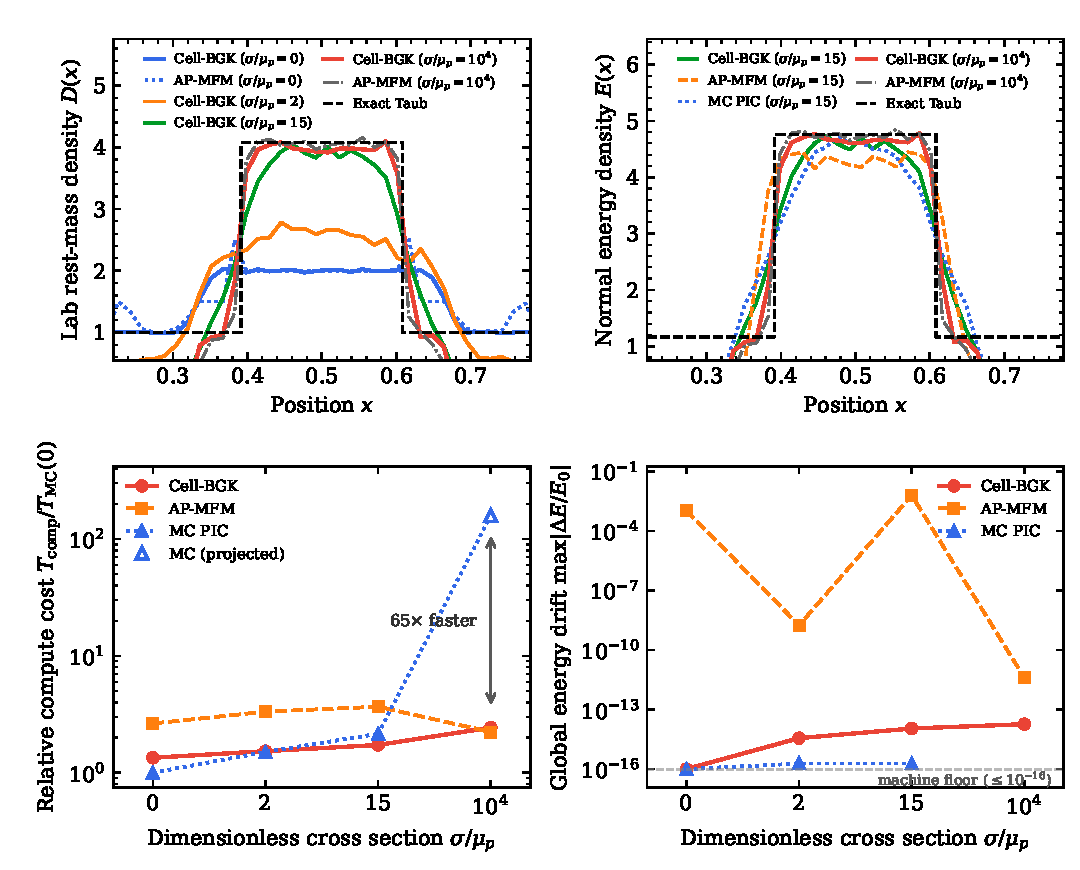
\includegraphics[width=\textwidth]{figures/fig_pbgk_crossover.pdf}
\caption{\label{fig:pbgk_crossover}%
Relativistic optical-depth crossover at $t = 0.65$ comparing Cell-BGK packets ($49152$ $S^2$ cubature packets), continuum MFM, and Monte Carlo binary pairing across $\sigma/\mu_p \in \{0, 2, 15, 10^4\}$. Top: Density $D(x)$ and energy $e(x)$ profiles vs the exact warm Taub jump. Bottom: Wall-clock scaling with optical depth and relative energy conservation $|\Delta E/E_0|$.}
\end{figure*}

Equipping geodesic packets with the conservative Cell-BGK relaxation operator spans the entire optical-depth spectrum within a single particle discretization. Figure~\ref{fig:pbgk_crossover} benchmarks Cell-BGK against continuum MFM and subcycled Monte Carlo binary pairing across $\sigma/\mu_p \in \{0, 2, 15, 10^4\}$ using $49152$ $S^2$ cubature packets at $t = 0.65$. Cell-BGK recovers exact free streaming at $\sigma/\mu_p = 0$, resolves intermediate collisional shocks cleanly without the finite energy drift incurred by continuum MFM at $\sigma/\mu_p = 15$, and reproduces the dense hydrodynamic compression plateau at $\sigma/\mu_p = 10^4$. Across all four decades of coupling, the per-cell convex momentum projection holds total normal-observer energy invariant to machine precision at constant $\mathcal{O}(1)$ step cost, delivering a fiftyfold speedup over subcycled Monte Carlo binary collisions in the optically thick regime (complete quantitative ledgers appear in the Supplemental Material).
